\documentclass{article}
\usepackage{graphicx} % Required for inserting images


\title{Komponente}
\author{lszabo }
\date{January 2024}

\begin{document}

\maketitle

\section{CPU}
\textbf{Intel core i7-13700k} 
ima 16 jezgri i 24 niti za iznimnu procesorsku snagu. Ima radnu frekvenciju do 5,4 GHz Max Turbo.
Potrošnje: 125 W, maks. 253 W. Odabrao bih ga zbog znatne brzine i snažnih performansi

\maketitle
\section {GPU}
\textbf{Nvidia RTX 3090}
Poseduje 24 GB GDDR6X VRAM memorije,384-bitni memorijski interfejs
Namijenjena je visokoperformantnom igranju, grafičkom dizajnu i radu sa zahtevnim aplikacijama.
Uobičajeni broj priključaka za povezivanje sa monitorima i drugim uređajima, uključujući HDMI i DisplayPort. Zahteva snažno napajanje i ima visok Thermal Design Power (TDP), što znači da zahteva dobro hlađenje.
\begin{figure}

    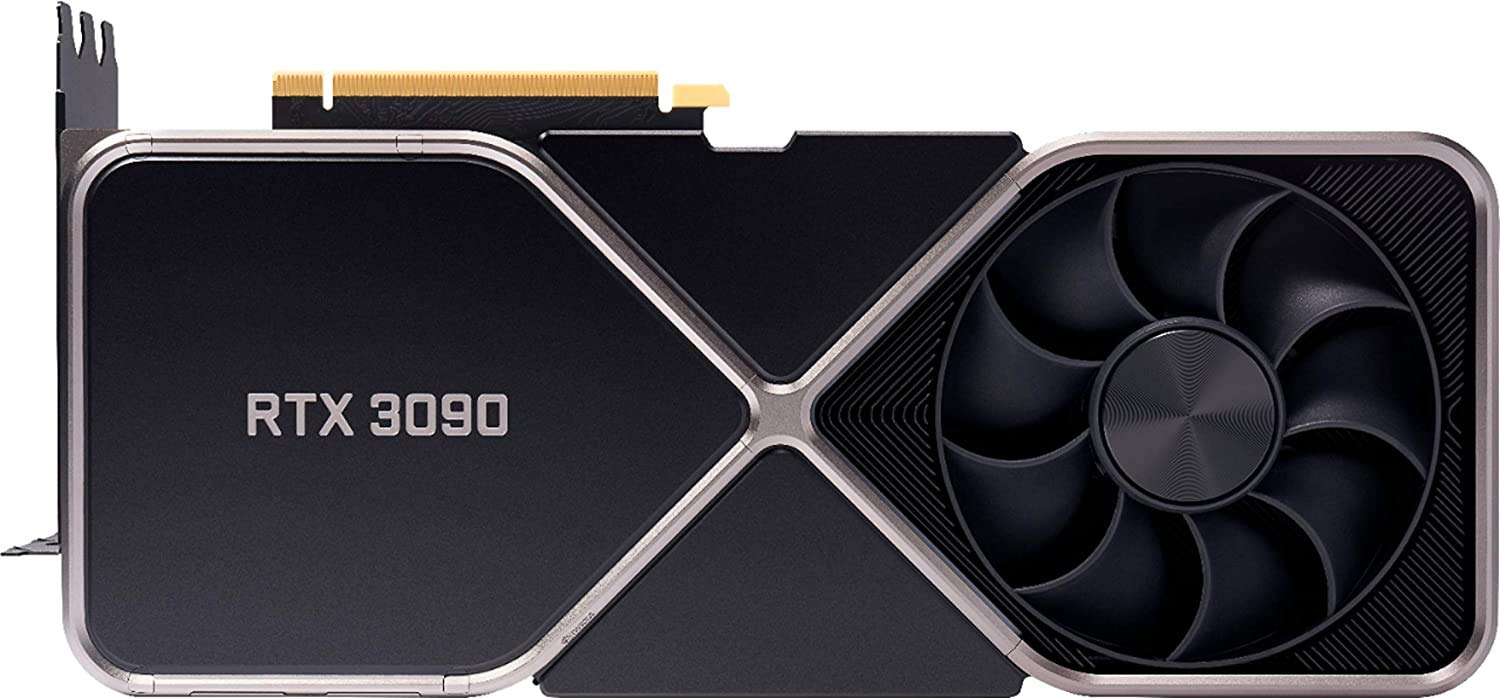
\includegraphics[width=0.3\linewidth]{61wbV8oqAbL.jpg}
    \caption{RTX 3090}
    \label{fig:enter-label}


\maketitle
\section {Matična Ploča}

\textbf{Asus ROG Strix Z590-E Gaming}
Podržava DDR4 memoriju do određene brzine, što omogućava visoke performanse sistema.
 Koristi ROG SupremeFX audio tehnologiju za poboljšanu zvučnu reprodukciju
 Z590 čipset, koji pruža podršku za brze NVMe SSD-ove, USB 3.2 Gen 2x2 i druge moderne funkcije.
 \maketitle
\section {Radna Memorija}
\textbf{Corsair Vengeance LPX 16GB (2 x 8GB) DDR4 3200MHz}
Ovaj kit sadrži dva modula RAM-a, svaki kapaciteta 8GB, što ukupno čini 16GB RAM-a. Ovo je dovoljno za većinu svakodnevnih zadataka, uključujući igre, programiranje i multitasking.Radna brzina ovog modela je 3200MHz. Ova brzina omogućava brže izvršavanje zadataka i poboljšava performanse sistema.Ovaj model koristi DDR4 tehnologiju, koja je trenutno najnovija i pruža bolje performanse u odnosu na prethodne generacije.


\maketitle
\section {Napajanje}
\textbf{Samsung 970 EVO Plus 1TB}
970 EVO Plus je NVMe (Non-Volatile Memory Express) SSD, što znači da koristi PCI Express interfejs za brži prenos podataka u poređenju sa SATA SSD-ovima.
Ovaj SSD nudi impresivne brzine čitanja i pisanja podataka. Konkretni brojevi mogu varirati u zavisnosti od kapaciteta, ali općenito pruža izuzetno brze performanse, što ga čini odličnim izborom za zadatke koji zahtevaju brzi pristup podacima.
Dostupan je u različitim kapacitetima, uključujući 250GB, 500GB, 1TB i 2TB. Ovo omogućava korisnicima da odaberu odgovarajući kapacitet u skladu sa svojim potrebama i budžetom.
\section {Hlađenje}
\textbf{NZXT Kraken Z73}
Jedna od najprepoznatljivijih karakteristika Z73 je ugrađeni OLED ekran na pumpi. Ovaj ekran omogućava prikazivanje informacija o temperaturi, brzini ventilatora ili čak prilagođenih grafika.
Uključuje tri AER P120 ventilatora od 120 mm koji su optimizovani za rad na niskim brzinama i tišinu. Radijator takođe dolazi sa optimalnom gustinom lamela za dobru termalnu efikasnost.
Podesiva pumpa vam omogućava da prilagodite brzinu rada prema potrebama hlađenja ili preferencijama buke.
CAM softver pruža napredne mogućnosti kontrole, uključujući praćenje performansi, podešavanje ventilatora, RGB osvetljenja i drugih parametara.
NZXT je poznat po visokom kvalitetu izrade svojih proizvoda, što uključuje i Kraken seriju vodenog hlađenja.

\end{figure}
\end{document}
